\section{Evaluation}%
\label{sec:evaluation}

We answer $RQ_2$ by evaluating our enclave framework with respect to
security (\S~\ref{sec:security}),
financial cost (\S~\ref{sec:cost}), and performance.  As for performance, we
study the rate at which one can generate
attestation documents (\S~\ref{sec:attestation-performance}),
application latency (\S~\ref{sec:latency}),
and application throughput (\S~\ref{sec:throughput}).

We ran our performance measurements on a c5.xlarge EC2 host, which is on the
lower end of enclave-capable instance types.  Our performance numbers therefore
represent a lower bound of what's possible.  More powerful (and therefore more
expensive) instance types result in better performance.

\subsection{Security considerations}%
\label{sec:security}

There are three key components to the overall security of an enclave
application:
(i) Amazon's Nitro system itself,
(ii) \tool{}, and
(iii) the application that runs on top of \tool{}.

The security foundation lies in the soundness of the design of Nitro enclaves.
While Amazon published the conceptual design~\cite{Bean2022a}, the concrete
hardware and software implementation is closed source.  The decision to
allocate physically separate resources to enclaves appears promising but only
time will tell if Nitro enclaves can resist the types of attacks that have been
plaguing SGX.  If we assume that Nitro enclaves are acceptably secure, the next
component is \tool{}.

\Tool{}'s security reduces to the complexity of our code and the security of its
cryptographic building blocks.  These building blocks are SHA-256 (to hash
public key material that is embedded in the attestation document), the NaCl
cryptographic library~\cite{nacl} (to implement key
synchronization),\footnote{Specifically, we use NaCl's box API, which uses
Curve25519, XSalsa20, and Poly1305 to encrypt and authenticate messages.} TLS in
at least version 1.2 (to provide a secure channel between clients and the
enclave), and Go's CSPRNG, which is seeded with randomness from the Nitro
hypervisor.
% ls -1 *.go | grep -v "_test.go" | xargs wc -l
One measure of our code complexity is its size.  Excluding unit tests, \tool{}
counts less than 1,700 lines of code and has nine direct dependencies
that are not maintained by either us or the Go project.\footnote{Most
dependencies provide networking functionality like a user-space TCP stack, code
that provides a TAP interface, and a wrapper for Linux's netlink interface.}
%
Nine is worse than zero, but is still manageable and auditable in its entirety.
Our choice of using Go and the (comparatively) small trusted computing base
greatly reduces---but does not eliminate!---the attack surface.

The highest layer in the software stack is the enclave application itself.  The
biggest security threat are side channel attacks and programming bugs.  It is
the application developer's responsibility to prevent side channel attacks and
write bug-free code.  As we pointed out in Section~\ref{sec:limitations},
programming bugs can be intentional, i.e., the service provider may deliberately
introduce bugs that leak sensitive information.  From the user's point of view,
eternal vigilance is therefore the price of security.

\subsection{Financial cost}%
\label{sec:cost}

Nitro enclaves do not incur any extra cost in addition to what the underlying
EC2 host costs---they can be considered a ``free'' extension to EC2.  Nitro
enclaves are however only available for select types of EC2 instances because
they require their own CPU and a minimum amount of memory, and those instance
types are pricier than the lowest tier that AWS offers.  We tested all of the
practical applications of Section~\ref{sec:applications} on a c5.xlarge
instance, which is on the lower end of enclave-enabled EC2 instance types.
This instance comes with four vCPUs and 8 GiB of memory.  As of March 2023, a
c5.xlarge instance costs USD 0.17 per hour, which amounts to approximately USD
125 per month.

\subsection{Attestation document request rate}%
\label{sec:attestation-performance}

The fetching of attestation documents is a critical part of our framework's
overall performance.  We built a stress test application that runs a busy loop
for 60 seconds to request as many attestation documents as possible.  For each
request, we ask the hypervisor to include an incrementing nonce in the
attestation document, to avoid any speedups by caching.
Table~\ref{tab:att-perf} shows the results.  We were able to obtain
approximately 840 documents per second with the median request taking 1.1
milliseconds to complete.

\begin{table}[t]
    \centering
    \begin{tabular}{r r r r}
    \toprule
      Min. (ms) & Median (ms) & Mean (ms) & Max. (ms) \\
    \midrule
      1.1 & 1.1 & 1.2 & 7.9 \\
    \bottomrule
    \end{tabular}
    \caption{Summary statistics capturing the expected latency of requesting
    attestation documents from the Nitro hypervisor.}%
    \label{tab:att-perf}
\end{table}

\subsection{Application latency}%
\label{sec:latency}

We seek to measure two types of latency: (i) the latency induced by the
interface between an EC2 host and its Nitro enclave and (ii) the latency induced
by \tool{}, both with and without \tool{}'s reverse proxy configuration.  We
built a lightweight enclave application that helps us measure these latencies.
The application implements a Web server that responds with the string ``hello
world'' upon receiving requests for its index page.  We made this application
minimal because we're only interested in the latency \emph{before} a request
reaches the enclave application.  We therefore also deactivate the Web server's
TLS support and use plain HTTP for our measurements.  To simulate clients, we
use the HTTP load test tool Baton~\cite{baton}.  Equipped with both an HTTP
server and client, we measure the request latency to our application in five
separate setups:

\begin{description}
  \item[Loopback] The client talks to the Web server via the loopback interface.
    This setup provides the latency baseline that we compare against.

  \item[Docker] The Web server runs in a local Docker container.

  \item[Enclave] The Web server runs inside a Nitro enclave but without \tool{}.
    All traffic goes over the VSOCK interface.  This measures the latency
    introduced by the interface to the Nitro enclave.

  \item[\Tool{}-nrp] The Web server runs inside a Nitro enclave but without a
    reverse proxy.  This measures the latency introduced by \tool{}'s tap
    forwarding code.

  \item[\Tool{}] The Web server runs inside a Nitro enclave with \tool{} acting
    as a reverse HTTP proxy.  This measures the latency introduced by \tool{}'s
    tap forwarding code \emph{and} its reverse HTTP proxy.
\end{description}

We run Baton on the parent EC2 host and instruct it to send 100,000 requests
using 10 concurrent threads.  We had to patch Baton's source code to add VSOCK
support (to be able to send requests directly to the enclave via the VSOCK
interface) and to log latency percentiles.  Note that our measurements
constitute a \emph{lower bound} of the latency that is achievable.  Real-world
applications will exhibit higher latency because clients send their requests
over the Internet (which adds considerable networking latency) and the enclave
application is likely to be more complex (which adds computational latency).

\begin{table}[t]
    \centering
    \begin{tabular}{l r r r}
    \toprule
      Setup & \makecell[r]{Requests\\(per sec)} &
              \makecell[r]{Mean latency\\(ms)} &
              \makecell[r]{Max latency\\(ms)} \\
    \midrule
      Loopback      & 40,913 &  0.06 & 20 \\
      Docker        & 19,321 &  0.12 & 15 \\
      Enclave       & 16,466 &  0.06 &  9 \\
      Nitriding-nrp &  2,288 &  3.74 & 53 \\
      Nitriding     &  1,214 &  7.63 & 63 \\
    \bottomrule
    \end{tabular}
    \caption{The number of HTTP requests per second when making requests from
    ten threads in parallel, and 100,000 requests in total.}%
    \label{tab:latency-msmts}
\end{table}

Table~\ref{tab:latency-msmts} illustrates the results.  The Web server can
sustain more than 40,000 requests per second over the loopback interface.  When
run inside a Docker container, we can achieve only half of that.  Running the
Web server inside an enclave instead of in a Docker container results in a 15\%
decrease in requests.  \Tool{} without a reverse proxy can sustain 14\% of the
enclave setup, and \tool{} with reverse proxy results in 1,214 requests per
second---7\% of what's possible in the pure-enclave setup.  We attribute this
slowdown primarily to our use of a user-space TCP stack.
Figure~\ref{fig:latency-cdf} shows the empirical CDF of the response latency
for our Web request measurement.

\begin{figure}[t]
    \centering
    % Created by tikzDevice version 0.12.3.1 on 2023-02-04 10:22:28
% !TEX encoding = UTF-8 Unicode
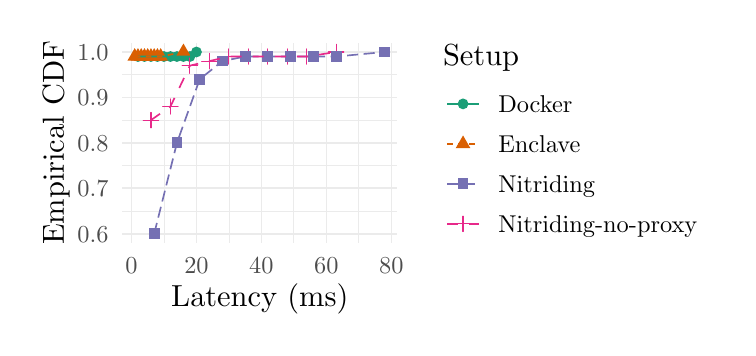
\begin{tikzpicture}[x=1pt,y=1pt]
\definecolor{fillColor}{RGB}{255,255,255}
\path[use as bounding box,fill=fillColor,fill opacity=0.00] (0,0) rectangle (252.94,108.41);
\begin{scope}
\path[clip] ( 34.16, 30.69) rectangle (133.59,102.90);
\definecolor{drawColor}{gray}{0.92}

\path[draw=drawColor,line width= 0.3pt,line join=round] ( 34.16, 42.18) --
	(133.59, 42.18);

\path[draw=drawColor,line width= 0.3pt,line join=round] ( 34.16, 58.59) --
	(133.59, 58.59);

\path[draw=drawColor,line width= 0.3pt,line join=round] ( 34.16, 75.00) --
	(133.59, 75.00);

\path[draw=drawColor,line width= 0.3pt,line join=round] ( 34.16, 91.42) --
	(133.59, 91.42);

\path[draw=drawColor,line width= 0.3pt,line join=round] ( 49.24, 30.69) --
	( 49.24,102.90);

\path[draw=drawColor,line width= 0.3pt,line join=round] ( 72.72, 30.69) --
	( 72.72,102.90);

\path[draw=drawColor,line width= 0.3pt,line join=round] ( 96.20, 30.69) --
	( 96.20,102.90);

\path[draw=drawColor,line width= 0.3pt,line join=round] (119.68, 30.69) --
	(119.68,102.90);

\path[draw=drawColor,line width= 0.6pt,line join=round] ( 34.16, 33.97) --
	(133.59, 33.97);

\path[draw=drawColor,line width= 0.6pt,line join=round] ( 34.16, 50.38) --
	(133.59, 50.38);

\path[draw=drawColor,line width= 0.6pt,line join=round] ( 34.16, 66.80) --
	(133.59, 66.80);

\path[draw=drawColor,line width= 0.6pt,line join=round] ( 34.16, 83.21) --
	(133.59, 83.21);

\path[draw=drawColor,line width= 0.6pt,line join=round] ( 34.16, 99.62) --
	(133.59, 99.62);

\path[draw=drawColor,line width= 0.6pt,line join=round] ( 37.50, 30.69) --
	( 37.50,102.90);

\path[draw=drawColor,line width= 0.6pt,line join=round] ( 60.98, 30.69) --
	( 60.98,102.90);

\path[draw=drawColor,line width= 0.6pt,line join=round] ( 84.46, 30.69) --
	( 84.46,102.90);

\path[draw=drawColor,line width= 0.6pt,line join=round] (107.94, 30.69) --
	(107.94,102.90);

\path[draw=drawColor,line width= 0.6pt,line join=round] (131.42, 30.69) --
	(131.42,102.90);
\definecolor{fillColor}{RGB}{27,158,119}

\path[fill=fillColor] ( 39.85, 97.98) circle (  1.96);

\path[fill=fillColor] ( 42.20, 97.98) circle (  1.96);

\path[fill=fillColor] ( 44.55, 97.98) circle (  1.96);

\path[fill=fillColor] ( 46.89, 97.98) circle (  1.96);

\path[fill=fillColor] ( 49.24, 97.98) circle (  1.96);

\path[fill=fillColor] ( 51.59, 97.98) circle (  1.96);

\path[fill=fillColor] ( 53.94, 97.98) circle (  1.96);

\path[fill=fillColor] ( 56.29, 97.98) circle (  1.96);

\path[fill=fillColor] ( 58.63, 97.98) circle (  1.96);

\path[fill=fillColor] ( 60.98, 99.62) circle (  1.96);
\definecolor{fillColor}{RGB}{217,95,2}

\path[fill=fillColor] ( 38.68,101.03) --
	( 41.32, 96.46) --
	( 36.03, 96.46) --
	cycle;

\path[fill=fillColor] ( 39.85,101.03) --
	( 42.49, 96.46) --
	( 37.21, 96.46) --
	cycle;

\path[fill=fillColor] ( 41.02,101.03) --
	( 43.67, 96.46) --
	( 38.38, 96.46) --
	cycle;

\path[fill=fillColor] ( 42.20,101.03) --
	( 44.84, 96.46) --
	( 39.56, 96.46) --
	cycle;

\path[fill=fillColor] ( 43.37,101.03) --
	( 46.01, 96.46) --
	( 40.73, 96.46) --
	cycle;

\path[fill=fillColor] ( 44.55,101.03) --
	( 47.19, 96.46) --
	( 41.90, 96.46) --
	cycle;

\path[fill=fillColor] ( 45.72,101.03) --
	( 48.36, 96.46) --
	( 43.08, 96.46) --
	cycle;

\path[fill=fillColor] ( 46.89,101.03) --
	( 49.54, 96.46) --
	( 44.25, 96.46) --
	cycle;

\path[fill=fillColor] ( 48.07,101.03) --
	( 50.71, 96.46) --
	( 45.43, 96.46) --
	cycle;

\path[fill=fillColor] ( 56.29,102.67) --
	( 58.93, 98.10) --
	( 53.64, 98.10) --
	cycle;
\definecolor{drawColor}{RGB}{231,41,138}

\path[draw=drawColor,line width= 0.4pt,line join=round,line cap=round] ( 41.77, 75.00) -- ( 47.32, 75.00);

\path[draw=drawColor,line width= 0.4pt,line join=round,line cap=round] ( 44.55, 72.23) -- ( 44.55, 77.78);

\path[draw=drawColor,line width= 0.4pt,line join=round,line cap=round] ( 48.81, 79.93) -- ( 54.36, 79.93);

\path[draw=drawColor,line width= 0.4pt,line join=round,line cap=round] ( 51.59, 77.15) -- ( 51.59, 82.70);

\path[draw=drawColor,line width= 0.4pt,line join=round,line cap=round] ( 55.86, 94.70) -- ( 61.41, 94.70);

\path[draw=drawColor,line width= 0.4pt,line join=round,line cap=round] ( 58.63, 91.92) -- ( 58.63, 97.47);

\path[draw=drawColor,line width= 0.4pt,line join=round,line cap=round] ( 62.90, 96.34) -- ( 68.45, 96.34);

\path[draw=drawColor,line width= 0.4pt,line join=round,line cap=round] ( 65.68, 93.56) -- ( 65.68, 99.11);

\path[draw=drawColor,line width= 0.4pt,line join=round,line cap=round] ( 69.95, 97.98) -- ( 75.50, 97.98);

\path[draw=drawColor,line width= 0.4pt,line join=round,line cap=round] ( 72.72, 95.21) -- ( 72.72,100.76);

\path[draw=drawColor,line width= 0.4pt,line join=round,line cap=round] ( 76.99, 97.98) -- ( 82.54, 97.98);

\path[draw=drawColor,line width= 0.4pt,line join=round,line cap=round] ( 79.77, 95.21) -- ( 79.77,100.76);

\path[draw=drawColor,line width= 0.4pt,line join=round,line cap=round] ( 84.03, 97.98) -- ( 89.58, 97.98);

\path[draw=drawColor,line width= 0.4pt,line join=round,line cap=round] ( 86.81, 95.21) -- ( 86.81,100.76);

\path[draw=drawColor,line width= 0.4pt,line join=round,line cap=round] ( 91.08, 97.98) -- ( 96.63, 97.98);

\path[draw=drawColor,line width= 0.4pt,line join=round,line cap=round] ( 93.85, 95.21) -- ( 93.85,100.76);

\path[draw=drawColor,line width= 0.4pt,line join=round,line cap=round] ( 98.12, 97.98) -- (103.67, 97.98);

\path[draw=drawColor,line width= 0.4pt,line join=round,line cap=round] (100.90, 95.21) -- (100.90,100.76);

\path[draw=drawColor,line width= 0.4pt,line join=round,line cap=round] (108.69, 99.62) -- (114.24, 99.62);

\path[draw=drawColor,line width= 0.4pt,line join=round,line cap=round] (111.46, 96.85) -- (111.46,102.40);
\definecolor{fillColor}{RGB}{117,112,179}

\path[fill=fillColor] ( 43.76, 32.01) --
	( 47.68, 32.01) --
	( 47.68, 35.93) --
	( 43.76, 35.93) --
	cycle;

\path[fill=fillColor] ( 51.98, 64.83) --
	( 55.90, 64.83) --
	( 55.90, 68.76) --
	( 51.98, 68.76) --
	cycle;

\path[fill=fillColor] ( 60.19, 87.81) --
	( 64.12, 87.81) --
	( 64.12, 91.74) --
	( 60.19, 91.74) --
	cycle;

\path[fill=fillColor] ( 68.41, 94.38) --
	( 72.34, 94.38) --
	( 72.34, 98.30) --
	( 68.41, 98.30) --
	cycle;

\path[fill=fillColor] ( 76.63, 96.02) --
	( 80.55, 96.02) --
	( 80.55, 99.94) --
	( 76.63, 99.94) --
	cycle;

\path[fill=fillColor] ( 84.85, 96.02) --
	( 88.77, 96.02) --
	( 88.77, 99.94) --
	( 84.85, 99.94) --
	cycle;

\path[fill=fillColor] ( 93.07, 96.02) --
	( 96.99, 96.02) --
	( 96.99, 99.94) --
	( 93.07, 99.94) --
	cycle;

\path[fill=fillColor] (101.28, 96.02) --
	(105.21, 96.02) --
	(105.21, 99.94) --
	(101.28, 99.94) --
	cycle;

\path[fill=fillColor] (109.50, 96.02) --
	(113.43, 96.02) --
	(113.43, 99.94) --
	(109.50, 99.94) --
	cycle;

\path[fill=fillColor] (127.11, 97.66) --
	(131.03, 97.66) --
	(131.03,101.58) --
	(127.11,101.58) --
	cycle;
\definecolor{drawColor}{RGB}{27,158,119}

\path[draw=drawColor,line width= 0.6pt,line join=round] ( 39.85, 97.98) --
	( 42.20, 97.98) --
	( 44.55, 97.98) --
	( 46.89, 97.98) --
	( 49.24, 97.98) --
	( 51.59, 97.98) --
	( 53.94, 97.98) --
	( 56.29, 97.98) --
	( 58.63, 97.98) --
	( 60.98, 99.62);
\definecolor{drawColor}{RGB}{217,95,2}

\path[draw=drawColor,line width= 0.6pt,dash pattern=on 2pt off 2pt ,line join=round] ( 38.68, 97.98) --
	( 39.85, 97.98) --
	( 41.02, 97.98) --
	( 42.20, 97.98) --
	( 43.37, 97.98) --
	( 44.55, 97.98) --
	( 45.72, 97.98) --
	( 46.89, 97.98) --
	( 48.07, 97.98) --
	( 56.29, 99.62);
\definecolor{drawColor}{RGB}{117,112,179}

\path[draw=drawColor,line width= 0.6pt,dash pattern=on 4pt off 2pt ,line join=round] ( 45.72, 33.97) --
	( 53.94, 66.80) --
	( 62.16, 89.77) --
	( 70.37, 96.34) --
	( 78.59, 97.98) --
	( 86.81, 97.98) --
	( 95.03, 97.98) --
	(103.25, 97.98) --
	(111.46, 97.98) --
	(129.07, 99.62);
\definecolor{drawColor}{RGB}{231,41,138}

\path[draw=drawColor,line width= 0.6pt,dash pattern=on 4pt off 4pt ,line join=round] ( 44.55, 75.00) --
	( 51.59, 79.93) --
	( 58.63, 94.70) --
	( 65.68, 96.34) --
	( 72.72, 97.98) --
	( 79.77, 97.98) --
	( 86.81, 97.98) --
	( 93.85, 97.98) --
	(100.90, 97.98) --
	(111.46, 99.62);
\end{scope}
\begin{scope}
\path[clip] (  0.00,  0.00) rectangle (252.94,108.41);
\definecolor{drawColor}{gray}{0.30}

\node[text=drawColor,anchor=base east,inner sep=0pt, outer sep=0pt, scale=  0.88] at ( 29.21, 30.94) {0.6};

\node[text=drawColor,anchor=base east,inner sep=0pt, outer sep=0pt, scale=  0.88] at ( 29.21, 47.35) {0.7};

\node[text=drawColor,anchor=base east,inner sep=0pt, outer sep=0pt, scale=  0.88] at ( 29.21, 63.77) {0.8};

\node[text=drawColor,anchor=base east,inner sep=0pt, outer sep=0pt, scale=  0.88] at ( 29.21, 80.18) {0.9};

\node[text=drawColor,anchor=base east,inner sep=0pt, outer sep=0pt, scale=  0.88] at ( 29.21, 96.59) {1.0};
\end{scope}
\begin{scope}
\path[clip] (  0.00,  0.00) rectangle (252.94,108.41);
\definecolor{drawColor}{gray}{0.30}

\node[text=drawColor,anchor=base,inner sep=0pt, outer sep=0pt, scale=  0.88] at ( 37.50, 19.68) {0};

\node[text=drawColor,anchor=base,inner sep=0pt, outer sep=0pt, scale=  0.88] at ( 60.98, 19.68) {20};

\node[text=drawColor,anchor=base,inner sep=0pt, outer sep=0pt, scale=  0.88] at ( 84.46, 19.68) {40};

\node[text=drawColor,anchor=base,inner sep=0pt, outer sep=0pt, scale=  0.88] at (107.94, 19.68) {60};

\node[text=drawColor,anchor=base,inner sep=0pt, outer sep=0pt, scale=  0.88] at (131.42, 19.68) {80};
\end{scope}
\begin{scope}
\path[clip] (  0.00,  0.00) rectangle (252.94,108.41);
\definecolor{drawColor}{RGB}{0,0,0}

\node[text=drawColor,anchor=base,inner sep=0pt, outer sep=0pt, scale=  1.10] at ( 83.87,  7.64) {Latency (ms)};
\end{scope}
\begin{scope}
\path[clip] (  0.00,  0.00) rectangle (252.94,108.41);
\definecolor{drawColor}{RGB}{0,0,0}

\node[text=drawColor,rotate= 90.00,anchor=base,inner sep=0pt, outer sep=0pt, scale=  1.10] at ( 13.08, 66.80) {Empirical CDF};
\end{scope}
\begin{scope}
\path[clip] (  0.00,  0.00) rectangle (252.94,108.41);
\definecolor{drawColor}{RGB}{0,0,0}

\node[text=drawColor,anchor=base west,inner sep=0pt, outer sep=0pt, scale=  1.10] at (150.09, 94.67) {Setup};
\end{scope}
\begin{scope}
\path[clip] (  0.00,  0.00) rectangle (252.94,108.41);
\definecolor{fillColor}{RGB}{27,158,119}

\path[fill=fillColor] (157.32, 80.87) circle (  1.96);
\end{scope}
\begin{scope}
\path[clip] (  0.00,  0.00) rectangle (252.94,108.41);
\definecolor{drawColor}{RGB}{27,158,119}

\path[draw=drawColor,line width= 0.6pt,line join=round] (151.54, 80.87) -- (163.10, 80.87);
\end{scope}
\begin{scope}
\path[clip] (  0.00,  0.00) rectangle (252.94,108.41);
\definecolor{fillColor}{RGB}{217,95,2}

\path[fill=fillColor] (157.32, 69.47) --
	(159.96, 64.89) --
	(154.68, 64.89) --
	cycle;
\end{scope}
\begin{scope}
\path[clip] (  0.00,  0.00) rectangle (252.94,108.41);
\definecolor{drawColor}{RGB}{217,95,2}

\path[draw=drawColor,line width= 0.6pt,dash pattern=on 2pt off 2pt ,line join=round] (151.54, 66.42) -- (163.10, 66.42);
\end{scope}
\begin{scope}
\path[clip] (  0.00,  0.00) rectangle (252.94,108.41);
\definecolor{fillColor}{RGB}{117,112,179}

\path[fill=fillColor] (155.36, 50.00) --
	(159.28, 50.00) --
	(159.28, 53.92) --
	(155.36, 53.92) --
	cycle;
\end{scope}
\begin{scope}
\path[clip] (  0.00,  0.00) rectangle (252.94,108.41);
\definecolor{drawColor}{RGB}{117,112,179}

\path[draw=drawColor,line width= 0.6pt,dash pattern=on 4pt off 2pt ,line join=round] (151.54, 51.96) -- (163.10, 51.96);
\end{scope}
\begin{scope}
\path[clip] (  0.00,  0.00) rectangle (252.94,108.41);
\definecolor{drawColor}{RGB}{231,41,138}

\path[draw=drawColor,line width= 0.4pt,line join=round,line cap=round] (154.54, 37.51) -- (160.09, 37.51);

\path[draw=drawColor,line width= 0.4pt,line join=round,line cap=round] (157.32, 34.73) -- (157.32, 40.28);
\end{scope}
\begin{scope}
\path[clip] (  0.00,  0.00) rectangle (252.94,108.41);
\definecolor{drawColor}{RGB}{231,41,138}

\path[draw=drawColor,line width= 0.6pt,dash pattern=on 4pt off 4pt ,line join=round] (151.54, 37.51) -- (163.10, 37.51);
\end{scope}
\begin{scope}
\path[clip] (  0.00,  0.00) rectangle (252.94,108.41);
\definecolor{drawColor}{RGB}{0,0,0}

\node[text=drawColor,anchor=base west,inner sep=0pt, outer sep=0pt, scale=  0.88] at (170.05, 77.84) {Docker};
\end{scope}
\begin{scope}
\path[clip] (  0.00,  0.00) rectangle (252.94,108.41);
\definecolor{drawColor}{RGB}{0,0,0}

\node[text=drawColor,anchor=base west,inner sep=0pt, outer sep=0pt, scale=  0.88] at (170.05, 63.38) {Enclave};
\end{scope}
\begin{scope}
\path[clip] (  0.00,  0.00) rectangle (252.94,108.41);
\definecolor{drawColor}{RGB}{0,0,0}

\node[text=drawColor,anchor=base west,inner sep=0pt, outer sep=0pt, scale=  0.88] at (170.05, 48.93) {Nitriding};
\end{scope}
\begin{scope}
\path[clip] (  0.00,  0.00) rectangle (252.94,108.41);
\definecolor{drawColor}{RGB}{0,0,0}

\node[text=drawColor,anchor=base west,inner sep=0pt, outer sep=0pt, scale=  0.88] at (170.05, 34.48) {Nitriding-no-proxy};
\end{scope}
\end{tikzpicture}

    \caption{The empirical CDF of the latency distributions of our three test
      setups.}\label{fig:latency-cdf}
\end{figure}

\begin{table}[t]
    \centering
    \begin{tabular}{l r r}
    \toprule
      Setup & C $\rightarrow$ S (Gbits/sec) & S $\rightarrow$ C (Gbit/sec) \\
    \midrule
      Loopback        & 57.0 & 57.0 \\
      Docker          & 26.0 & 28.9 \\
      Enclave         &  3.6 &  3.2 \\
      Nitriding(-nrp) &  0.3 &  1.1 \\
    \bottomrule
    \end{tabular}
    \caption{The TCP throughput measurements when running iperf3 over the
    loopback interface, in Docker, inside an enclave, or inside an enclave using
    nitriding.}%
    \label{tab:iperf3}
\end{table}

\subsection{Application throughput}%
\label{sec:throughput}

Next, we measure the throughput that we can achieve over the VSOCK interface.
To that end, we use a VSOCK-enabled fork of the iperf3 performance measurement
tool in git commit \texttt{9245f9a}~\cite{iperf-vsock}.  iperf3 measures the
throughput of a networking link using a client/server model.  In our
experiment, we start an iperf3 server instance inside the enclave and the
corresponding client instance on the parent EC2 host.\footnote{The command that
we ran on the server was ``\texttt{iperf3 -{}-vsock -s}'' and on the client
``\texttt{iperf3 -{}-vsock -c 4}.''} The client then talks to the server via
the VSOCK interface and determines the maximum possible throughput.

When running both the iperf3 client \emph{and} server on the EC2 host---which
effectively measures the throughput of the EC2 host's loopback interface---we
achieve 57 GBit/s of throughput.  Running the iperf3 server inside a Docker
container reduces throughput to approximately 27 Gbit/s.  The enclave interface
further limits throughput to 3 Gbit/s while \tool{} results in approximately
0.3 Gbit/s.
